\subsection{Interruzione del Monitoraggio}\label{Interruzione}

Una volta avviato correttamente il monitoraggio dei dati di una certa rete bayesiana (§\ref{Avvio}) l'utente può, ovviamente, interrompere tale monitoraggio quando lo desidera.\\
Per far ciò l'utente deve trovarsi nella sezione del plug-in dedicata alle Impostazioni di Collegamento. Tale sezione è quella "principale", ovvero quella dove l'utente si trova fin dall'inizio. Nel caso l'utente si trovi nella sezione deputata alla visualizzazione dei monitoraggi attivi egli può facilmente accedere alla impostazioni di collegamento tramite l'operazione apposita (§\ref{ImpostazioniCollegamento}).\\
L'utente devi quindi selezionare, e dunque caricare sul pannello, la rete bayesiana di cui desidera interrompere il monitoraggio. Tale funzionalità è descritta in §\ref{SelezioneRete}.\\
~\\
L'operazione vera e propria di interruzione di monitoraggio consta dunque di un unico passaggio. È infatti sufficiente che l'utente clicchi il pulsante \textbf{Interrompi Monitoraggio}, visibile in Figura \ref{InterruzioneMonitoraggio}.

\begin{figure}[H]
	\begin{center}
		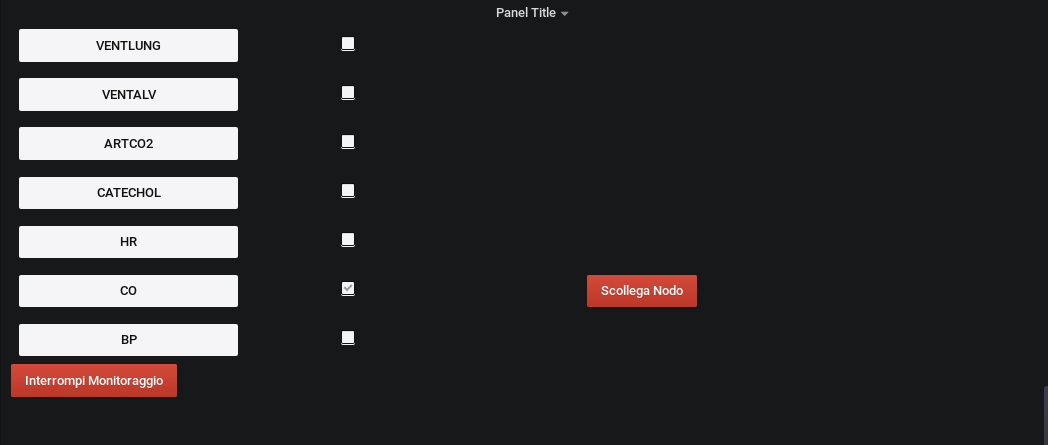
\includegraphics[scale=0.4]{./images/InterruzioneMonitoraggio.png}
		 \caption{Pulsante di Interruzione del Monitoraggio}	
		 \label{InterruzioneMonitoraggio}
	\end{center}
\end{figure}

Si noti che, nel caso in cui l'utente stia visualizzando una rete bayesiana non in fase di monitoraggio attivo, il pulsante \textbf{Interrompi Monitoraggio} non è presente. L'utente in quel caso infatti visualizzerà il pulsante \textbf{Avvia Monitoraggio} (Figura \ref{AvvioMonitoraggio}).\\
~\\
A seguito dell'interruzione del monitoraggio l'utente viene avvisato del buon esito dell'operazione attraverso un messaggio di notifica (Figura \ref{NotificaInterruzione}). La rete bayesiana, pur restando memorizzata nel server, non viene più monitorata, di conseguenza non è più possibile visualizzare i suoi dati di monitoraggio (§\ref{VisualDati})

\begin{figure}[H]
	\begin{center}
		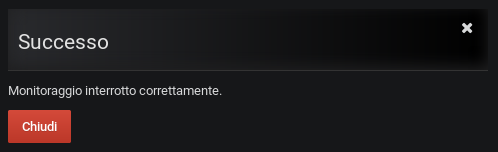
\includegraphics[scale=0.6]{./images/NotificaInterruzione.png}
		 \caption{Notifica di Interruzione del Monitoraggio Dati}	
		 \label{NotificaInterruzione}
	\end{center}
\end{figure}
